\subsection{Planung}
Dieses Unterkapitel beschäftigt sich mit der theoretischen Planung der Applikation. Es wird auf verschiedene Modellierungssprachen und deren unterschiedliche Diagrammtypen eingegangen. 

\subsubsection{Unified Modeling Language (UML)}
Mithilfe von \acs{UML} können komplexe Sachverhalte aus der Realität verständlich und einfach in Form von mehreren Diagrammtypen dargestellt werden. Durch \acs{UML} können Modelle aus simplen Teilen wie Klassen, Interfaces, Assoziationen, Generalisierungen \ac{usw.} zusammengebaut werden. Um ein komplexes System zu verstehen, muss es aus mehreren Blickwinkeln betrachtet werden. \cite{booch:1999:uml}

\paragraph{Klassendiagramm}
Ein Klassendiagramm stellt ein abstraktes Abbild des Source Codes dar. Es werden Klassen, Interfaces, Methoden und die Beziehung zwischen eben diesen dargestellt. Mit einem Klassendiagramm wird die statische Sicht auf ein System beleuchtet. \cite{booch:1999:uml} \\
Zur besseren Planung wird vor Beginn der Entwicklung ein grobes Konzept der Applikation in Form eines Klassendiagramms entworfen, wodurch die spätere Implementierung für die Entwickler/innen vereinfacht wird. Bereits vor der Implementierung existiert somit ein Grundgerüst, von dem aus der Entwicklungsstart vereinfacht wird. 

\paragraph{Aktivitätsdiagramm}
Ein Aktivitätsdiagramm zeigt den schrittweisen Ablauf von bestimmten Funktionen der Anwendung. Eine Aktivität wird als eine Reihe von Aktionen bezeichnet. Aktionen können verzweigt oder linear ablaufen. Mithilfe von Aktivitätsdiagrammen wird die dynamische Sicht auf ein System dargestellt. \cite{booch:1999:uml} \\
Um die komplexen Abläufe verständlicher darzustellen, werden vor der Implementierung mehrere Aktivitätsdiagramme entworfen. Damit kann auf einen Blick festgestellt werden, welche möglichen Verzweigungen die Funktion aufweist. Anhand des Diagramms können somit auch besser abdeckende Tests entworfen werden. In Abbildung \ref{fig:act-day-planning} ist das Aktivitätsdiagramm des Abschnitts \enquote{Tagesplanung} dargestellt. Der Ablauf der Aktivität wurde bereits im \autoref{chap:day-planning} detailiert beschrieben.

\begin{figure}[H]
    \centering
	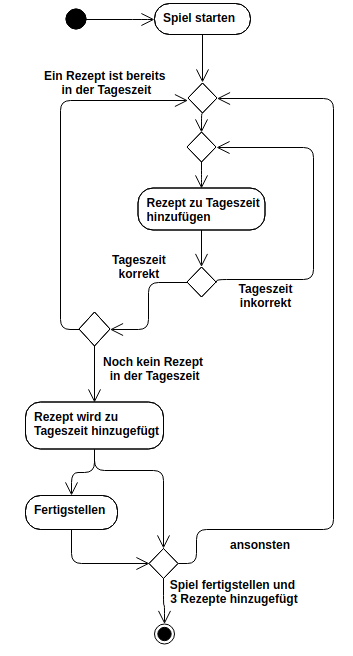
\includegraphics[width=0.4\linewidth]{figures/development/planning/activity/day-planning.png}
	\caption{Aktivitätsdiagramm für den Abschnitt \enquote{Tagesplanung}}
	\label{fig:act-day-planning}
\end{figure}

\subsubsection{Entity-Relationship-Modell (ERM)}
Das \acs{ERM} gehört zu den ältesten Modellen zur strukturierten Modellierung von Daten. Eine Klasse in der Objektorientierung entspricht einem Entitätstyp des \acs{ERM}. Entity-Relationship-Diagramme und \acs{UML}-Klassendiagramme haben eine ähnliche Struktur, weswegen \\ \acl{ERM}e auf \acs{UML} abgebildet werden können, jedoch nicht umgekehrt. Der wichtigste Teil des Diagramms sind sogenannte Entitäten, womit Objekte (Gegenstände, Personen, \dots) gemeint sind, die eindeutig identifiziert werden können. Alle Entitäten haben Eigenschaften, denen ein Wertebereich zugeordnet werden kann. Zwischen den Entitäten können unterschiedliche Arten von Beziehungen (1:1, 1:n, n:m) bestehen, die festlegen, wie viele Objekte an einer Beziehung beteiligt sind. \cite{goll:2011:methods_architectures}

Im folgenden Abschnitt wird auf die wichtigsten Teile des finalen \acl{ERM}s eingegangen (siehe Abbildungen \ref{fig:er_users}, \ref{fig:er_recipes}, \ref{fig:er_sessions}). Die unterschiedlichen Entitäten, sowie ihre Beziehungen zueinander werden kurz beschrieben. Um doppelte Formulierungen zu vermeiden werden Attribute, die alle Objekte besitzen nicht beschrieben. Alle Tabellen verfügen über zwei Zeitstempel, die angeben, wann ein Eintrag in die Datenbank eingefügt \acs{bzw.} bearbeitet wurde. Des Weiteren besitzen fast alle Entitäten zur eindeutigen Identifikation eine eindeutige ID.

\begin{figure}[H]
	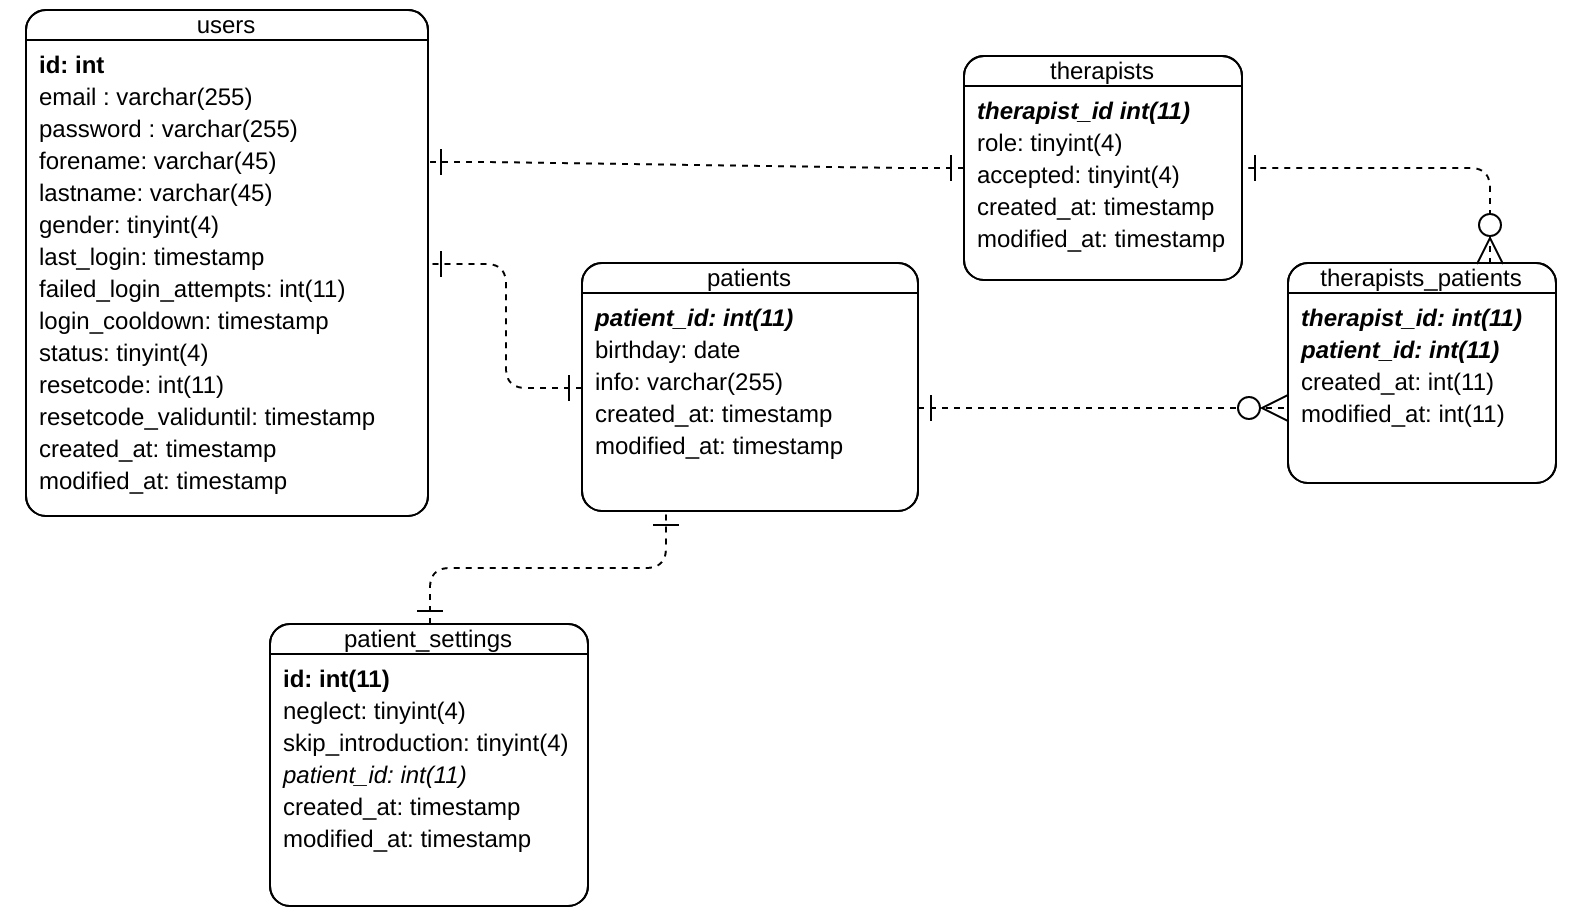
\includegraphics[width=1\linewidth]{figures/development/planning/er/users.png}
	\caption{Entitäten für die Benutzerverwaltung im \acs{ERM}}
	\label{fig:er_users}
\end{figure}

\paragraph{users}
Zu den zentralen Aspekten der Anwendung zählt die Benutzerverwaltung. Grundsätzlich wird die Applikation von Therapeut/innen und Patient/innen verwendet. Um gemeinsame Funktionen anbieten zu können, fungiert die \textit{users}-Entität als Elterntabelle für die \textit{therapists}- und \textit{patients}-Tabelle. Jede/r User/in kann sich registrieren, anmelden, Passwort zurücksetzen, Profil bearbeiten \acl{usw.}. Spezielle Eigenschaften, welche die Patient/innen und Therapeut/innen haben müssen, werden in den jeweiligen Entitäten beschrieben.

Die wichtigsten Attribute des/der Benutzer/in sind das Passwort und die E-Mail um den Zugang zur Applikation bereitzustellen. Weitere wichtige Attribute sind der Vor- sowie der Nachname und das Geschlecht des/der Anwender/in, damit zwischen den Nutzer/innen unterschieden werden kann. Die Eigenschaften \textit{failed\_login\_attempts} und \textit{login\_cooldown} dienen dazu, dass im Falle eines Missbrauchs des Accounts der/die User/in eine Zeit lang gesperrt werden kann. Die Möglichkeit das Passwort zurückzusetzen, wird durch die Felder \textit{resetcode} und \textit{resetcode\_validuntil} realisiert.

\paragraph{therapists}
Alle Therapeut/innen werden in dieser Tabelle gespeichert. Zusätzlich zu normalen Benutzer/innen müssen Therapeuten nach der Registrierung durch einen Administrator akzeptiert werden (\textit{accepted)}. Anhand der Rolle (\textit{role}) wird festgelegt, ob der Anwender/in ein Admin ist.

\paragraph{patients}
Alle Patienten werden in diesem Objekt abgelegt. Therapierende haben die Möglichkeit weitere Informationen zu den Behandelten zu speichern (\textit{info}), die wiederum von anderen Therapeut/innen abgerufen werden können. Darüber hinaus besitzt der/die Patient/in ein Geburtsdatum, da das Alter für die Therapie relevant sein könnte.

\paragraph{patient\_settings}
Diese Entität beinhaltet Einstellungen, die ein/e Patient/in treffen kann. Die Einstellungen können sich auf das gesamte Spiel auswirken. Dieses Objekt steht in direkter Beziehung (1:1) zum Behandelten.

Die Patient/innen-Einstellungen beinhalten beispielsweise eine Option (\textit{neglect}), ob der/die Betroffene an einem Neglect leidet. Für erfahrene Spieler/innen existiert das Feld \textit{skip\_introduction}, welches erlaubt, dass die Erklärung am Anfang des Spiels übersprungen wird.

\paragraph{therapists\_patients}
Am wichtigsten für die Behandlung ist die Zuweisung von Patient/innen an Therapeut/innen. Die beiden Entitäten (\textit{therapists}, \textit{patients}) sind jeweils mit einer 1:n-Beziehung mit diesem Objekt verbunden. Dies bedeutet, dass ein Therapierender mehrere Patient/innen haben kann und umgekehrt können Behandelte mehrere Therapeut/innen haben.

\begin{figure}[H]
	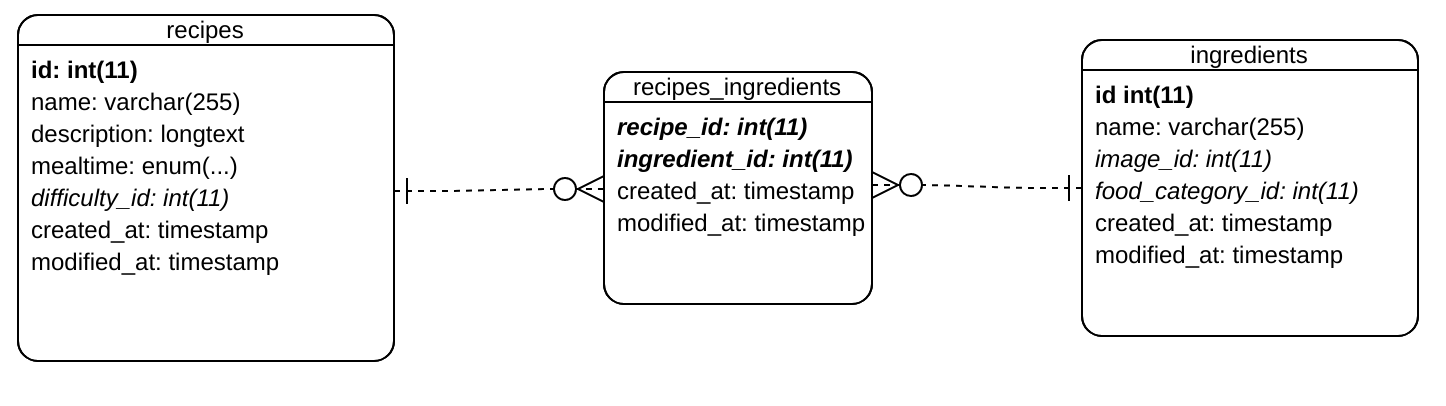
\includegraphics[width=1\linewidth]{figures/development/planning/er/recipes.png}
	\caption{Entitäten für die Rezeptverwaltung im \acs{ERM}}
	\label{fig:er_recipes}
\end{figure}

\paragraph{recipes}
Zentral für die Applikation sind die unterschiedlichen Rezepte. Diese Rezepte werden in dieser Entität festgehalten. Ein Rezept besitzt einen Namen, sowie eine Beschreibung zur Zubereitung. Zudem verfügt es über eine \textit{Tageszeit} (Frühstück, Mittag- und Abendessen) der Zubereitung und einen \textit{Schwierigskeitsgrad} (Leicht, Mittel, Schwer).
    
\paragraph{ingredients}
Die einzelnen Zutaten der Rezepten werden in der Entität \textit{ingredients} festgehalten. Eine Zutat hat einen \textit{Namen}, ein \textit{Bild} und eine \textit{Lebensmittelkategorie}.
    
\paragraph{recipes\_ingredients}
Die Zuweisung von Rezepten zu Zutaten werden in diesem Objekt festgehalten. Diese Entität steht in einer 1:n-Beziehung mit den Rezepten und Zutaten. Ein Rezept kann mehrere Zutaten haben und eine Zutaten kann in mehreren Rezepten enthalten sein.

\begin{figure}[H]
	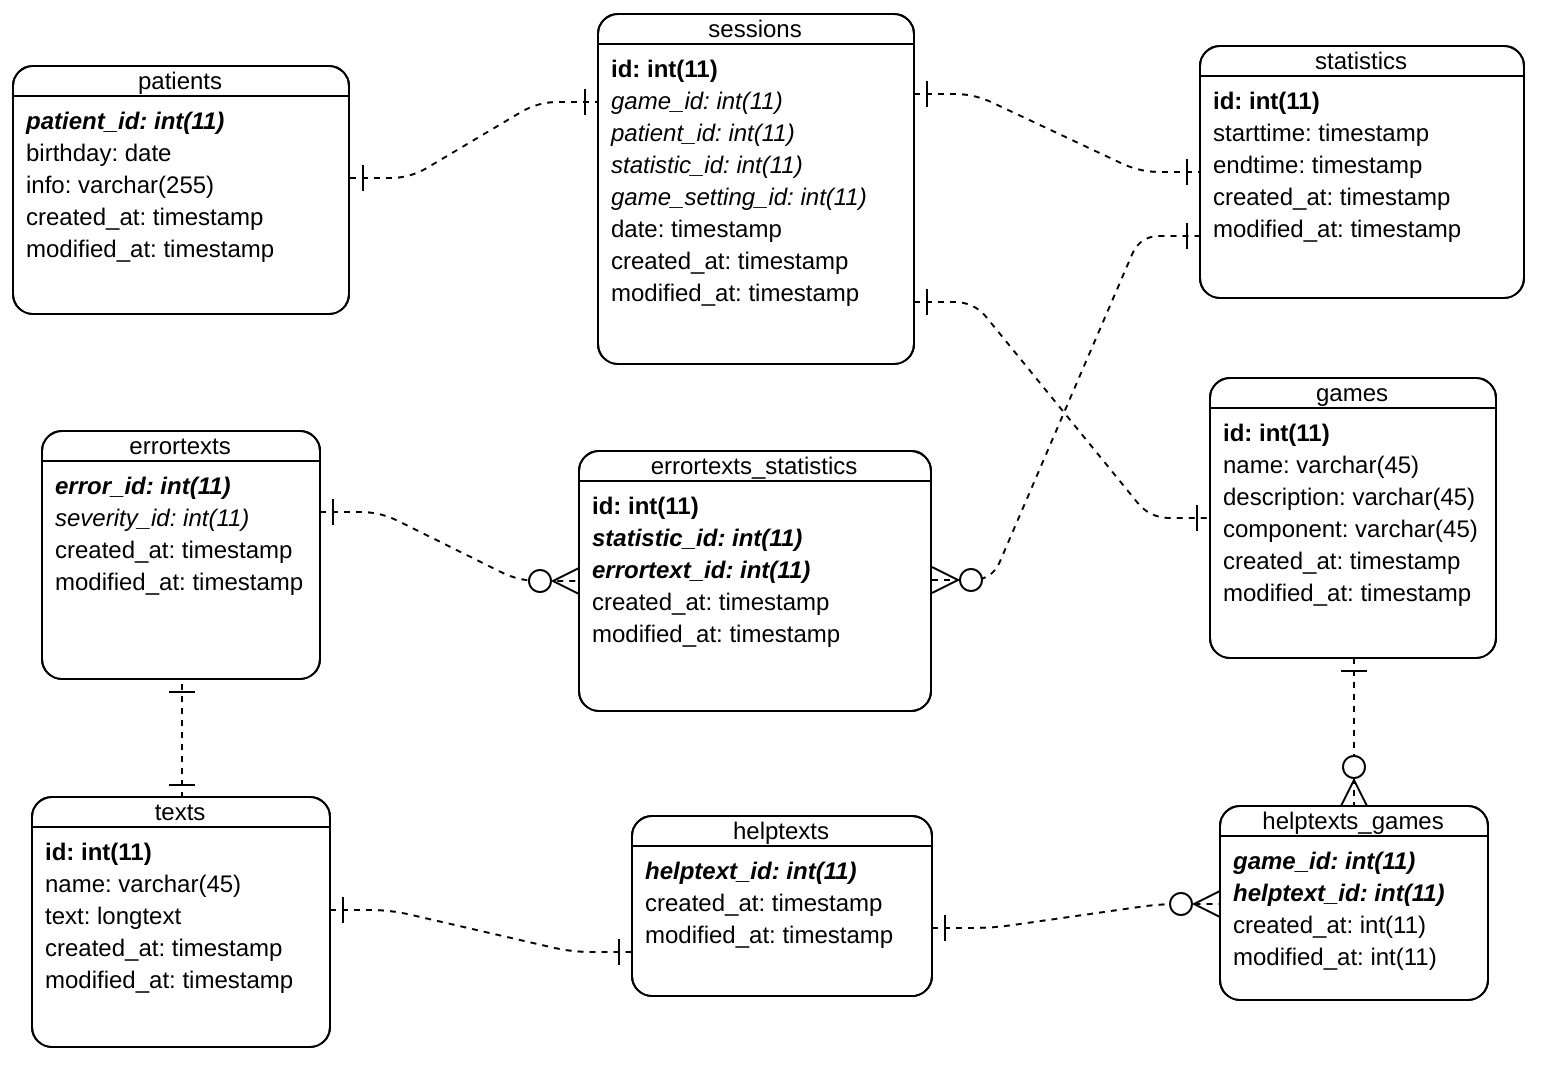
\includegraphics[width=1\linewidth]{figures/development/planning/er/sessions.png}
	\caption{Entitäten für die Sitzungsverwaltung im \acs{ERM}}
	\label{fig:er_sessions}
\end{figure}

\paragraph{sessions}
Im Mittelpunk der Applikation stehen die Spielsitzungen. Pro Sitzung werden wichtige Daten gesammelt, die den Therapieerfolg des/der Patient/in über die Zeit widerspiegeln sollen. Jede Session der Spieler/innen wird in der \textit{session}-Enität gespeichert. Die Patient/innen stehen in einer direkten Beziehung (1:1) mit der Session. In derselben Verbindung steht eine Sitzung mit der Entität \textit{Games}. Pro Session existiert eine Statistik.

Das Objekt besitzt noch einen \textit{Zeitpunkt}, an dem die Statistik stattgefunden hat. Dies dient dazu die Sitzung später eindeutig identifizieren zu können.
    
\paragraph{games}
Die verschiedenen Spiele der Applikation werden in dieser Entität abgelegt. Dieses Objekt steht wie oben bereits erwähnt, in einer 1:1 Beziehung mit der Session. Für jedes Spiel existieren mehrere Hilfetexte, daher steht die Entität mit der \textit{helptext\_games}-Entität in einer 1:n Beziehung.

Ein Spiel besitzt einen \textit{Namen} und eine kurze \textit{Beschreibung}. Zudem wird noch der Name der Komponente gespeichert. Dieser Umstand ist nur spiel-intern relevant.
    
\paragraph{statistics}
Die Zeiten pro Spiel und Sitzung werden in dieser Entität abgelegt. Die Statistik steht wie oben bereits beschrieben, in einer 1:1 Verbindung mit der Session. Pro Statistik, können noch mehrere Fehler gespeichert werden, die während des Spiels gemacht wurden. Jene Fehler werden in der Tabelle \textit{errortexts\_statistics} abgelegt.

Eine Statistik besitzt nur einen \textit{Start- und Endzeitpunkt}.
    
\paragraph{texts}
Jeder Abschnitt des Spiels beinhaltet Fehler- sowie Hilfetexte. Diese Texte werden in der \textit{texts}-Entität zusammengefasst. Dieses Objekt dient als übergeordnete Tabelle für \textit{errortexts} und \textit{helptexts}.

Jegliche Form von Text besitzt ein eindeutiges Kürzel (\textit{name}) und den eigentlichen Inhalt (\textit{text}) an sich. 
    
\paragraph{errortexts}
Die Fehlertexte sind eine Spezialisierung der Texte, welche in der Entität \textit{errortexts} zu finden sind. Für alle Arten von Fehlern existiert ein bereits vorgefertigter Text, der dem/der Spieler/in angezeigt wird, sobald diese/r einen Fehler gemacht hat. Das Objekt steht wie oben bereits beschrieben in einer Eltern-Kind Beziehung mit der Entität \textit{texts}.

Ein Fehlertext besitzt zusätzlich noch einen Schweregrad (\textit{severity}) der angibt, wie gravierend der Fehler für das Spiel war.
    
\paragraph{errortexts\_statistics}
Damit die Fehler pro Statistik abgelegt werden können wurde die Entität \textit{errortexts\_statistics} geschaffen. Ein Fehler kann in mehreren Statistiken vorkommen und eine Statistik kann mehrmals den gleichen Fehler haben. Im Nachhinein können sich beide Benutzer/innen-Gruppen alle Fehler mit Text pro Spiel und Sitzung ansehen.
    
\paragraph{helptexts}
Hilfetexte sind eine Ausprägung der Texte, welche in der Entität \textit{helptexts} festgehalten werden. Pro Spiel können mehrere Hilfetexte definiert werden, die dem/der Spieler/in den Einstieg erleichtern sollen, weshalb das Objekt in einer 1:n Verbindung mit der Entität \textit{helptexts\_games} steht. Wie zuvor bereits angemerkt wurde, stehen die Hilfetexte in einer 1:1 Beziehung mit der \textit{texts}-Entität, um auf den Inhalt des Texts zugreifen zu können.
    
\paragraph{helptexts\_games}
Die Zuordnung von Hilfetexten zu Spielen werden in dieser Entität abgelegt. Eine Hilfetext kann in mehreren Spielen vorkommen und ein Spiel kann mehrere Hilfetexte beinhalten, weshalb die \textit{helptexts}- und \textit{games}-Enitäten jeweils in einer 1:n Beziehung mit dem \textit{helptexts\_games} Objekt stehen.

